\section{Página de registro de usuarios}
\label{PRegistroUsuarios}

\begin{figure}[H]
\centerline{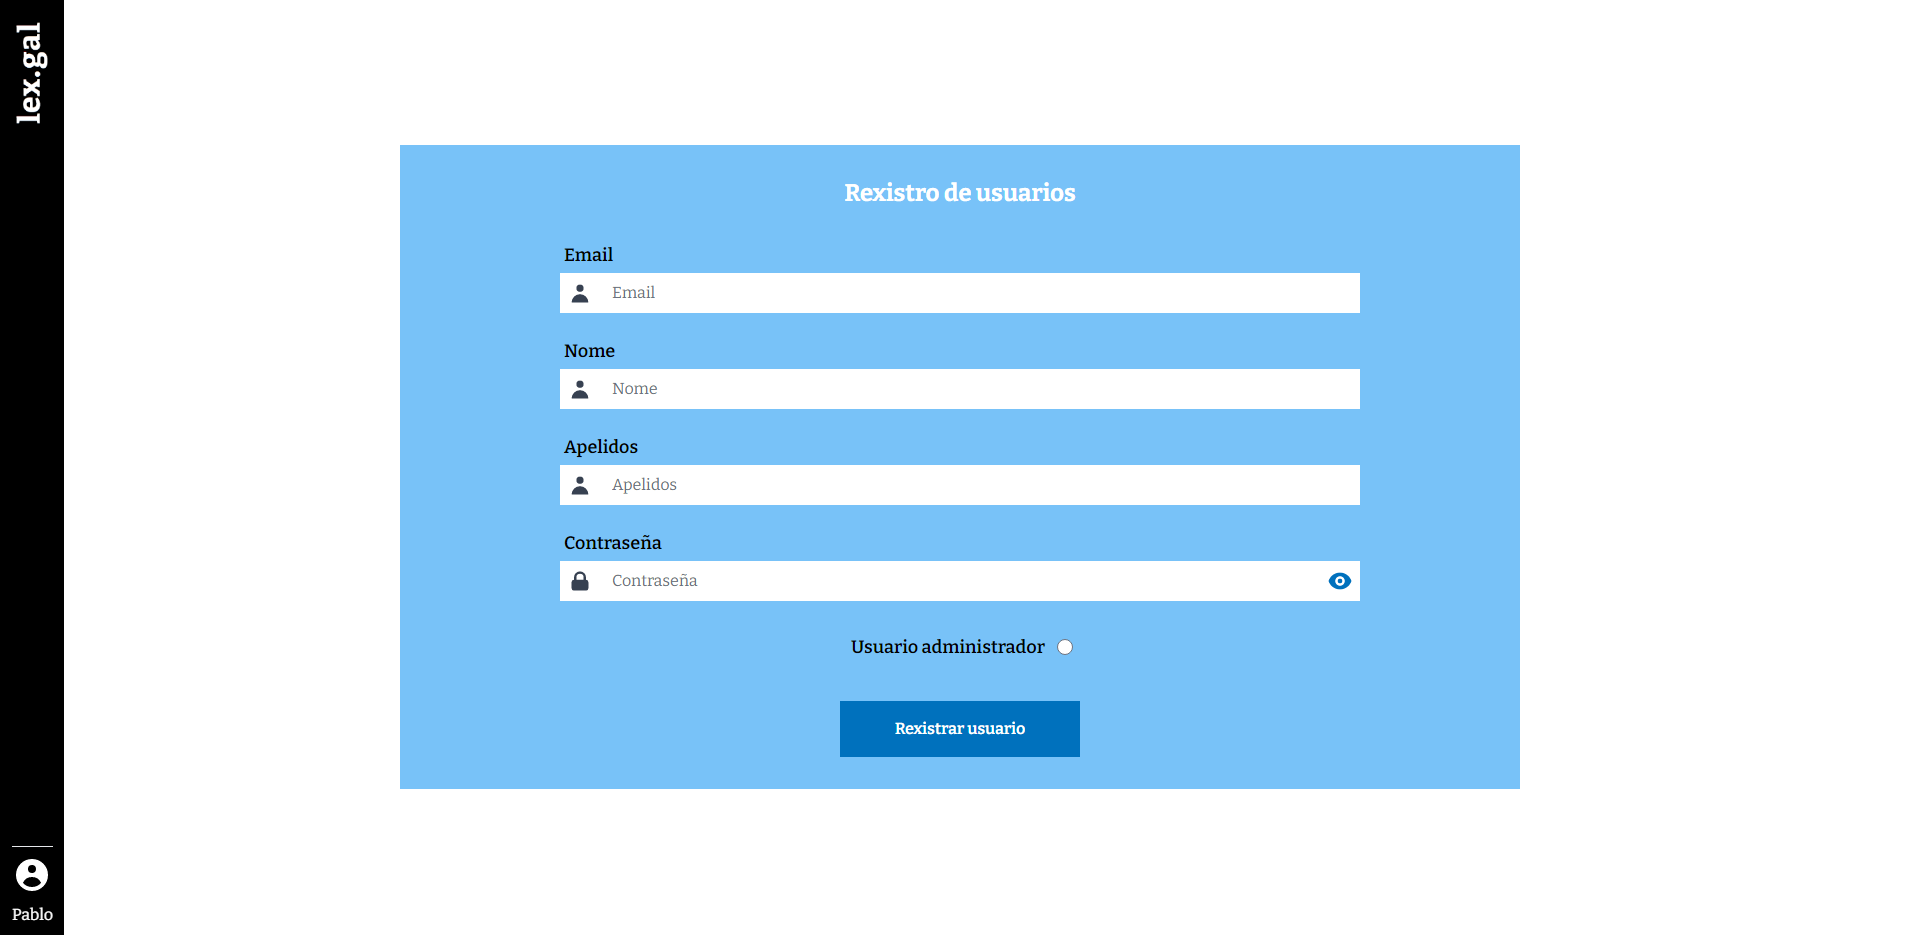
\includegraphics[width=12cm]{figuras/manualUsuario/RegistroUsuario.PNG}}
\caption{Página de registro de usuarios.}
\label{enlacePRegistroUsuarios}
\end{figure}

En esta página, que se ilustra en la \hyperref[enlacePRegistroUsuarios]{Figura B.4}, se permite el registro de usuarios, aunque esta solo puede ser accedida por usuarios administradores. En ella se puede introducir el correo electrónico, nombre, apellidos y contraseña. Por último, también se permite indicar si el usuario a registrar será administrador o no. Una vez se pincha en el botón de registrar usuario, se indica que el usuario ha sido registrado en la aplicación, y permite seguir registrando más usuarios.